        %%******************************************%%
        %%                                          %%
        %%        Modello di tesi di laurea         %%
        %%            di Andrea Giraldin            %%
        %%                                          %%
        %%             2 novembre 2012              %%
        %%                                          %%
        %%******************************************%%


% I seguenti commenti speciali impostano:
% 1. 
% 2. PDFLaTeX come motore di composizione;
% 3. tesi.tex come documento principale;
% 4. il controllo ortografico italiano per l'editor.

% !TEX encoding = UTF-8
% !TEX TS-program = pdflatex
% !TEX root = tesi.tex
% !TEX spellcheck = it-IT

\documentclass[10pt,                    % corpo del font principale
               a4paper,                 % carta A4
               twoside,                 % impagina per fronte-retro
               openright,               % inizio capitoli a destra
               english,                 
               italian,                 
               ]{book}    

%**************************************************************
% Importazione package
%************************************************************** 

%\usepackage{amsmath,amssymb,amsthm}    % matematica

\usepackage[T1]{fontenc}                % codifica dei font:
                                        % NOTA BENE! richiede una distribuzione *completa* di LaTeX

\usepackage[utf8]{inputenc}             % codifica di input; anche [latin1] va bene
                                        % NOTA BENE! va accordata con le preferenze dell'editor

\usepackage[english, italian]{babel}    % per scrivere in italiano e in inglese;
                                        % l'ultima lingua (l'italiano) risulta predefinita

\usepackage{bookmark}                   % segnalibri

\usepackage{caption}                    % didascalie

\usepackage{chngpage,calc}              % centra il frontespizio

\usepackage{csquotes}                   % gestisce automaticamente i caratteri (")

\usepackage{emptypage}                  % pagine vuote senza testatina e piede di pagina

\usepackage{epigraph}			% per epigrafi

\usepackage{eurosym}                    % simbolo dell'euro

%\usepackage{indentfirst}               % rientra il primo paragrafo di ogni sezione

\usepackage{graphicx}                   % immagini

\usepackage{hyperref}                   % collegamenti ipertestuali

\usepackage[binding=5mm]{layaureo}      % margini ottimizzati per l'A4; rilegatura di 5 mm

\usepackage{listings}                   % codici

\usepackage{microtype}                  % microtipografia

\usepackage{mparhack,fixltx2e,relsize}  % finezze tipografiche

\usepackage{nameref}                    % visualizza nome dei riferimenti                                      

\usepackage[font=small]{quoting}        % citazioni

\usepackage{subfig}                     % sottofigure, sottotabelle

\usepackage[italian]{varioref}          % riferimenti completi della pagina

\usepackage[dvipsnames]{xcolor}         % colori

\usepackage{booktabs}                   % tabelle                                       
\usepackage{tabularx}                   % tabelle di larghezza prefissata                                    
\usepackage{longtable}                  % tabelle su più pagine                                        
\usepackage{ltxtable}                   % tabelle su più pagine e adattabili in larghezza

\usepackage[toc, acronym]{glossaries}   % glossario
                                        % per includerlo nel documento bisogna:
                                        % 1. compilare una prima volta tesi.tex;
                                        % 2. eseguire: makeindex -s tesi.ist -t tesi.glg -o tesi.gls tesi.glo
                                        % 3. eseguire: makeindex -s tesi.ist -t tesi.alg -o tesi.acr tesi.acn
                                        % 4. compilare due volte tesi.tex.

\usepackage[backend=biber,style=verbose-ibid,hyperref,backref]{biblatex}
                                        % eccellente pacchetto per la bibliografia; 
                                        % produce uno stile di citazione autore-anno; 
                                        % lo stile "numeric-comp" produce riferimenti numerici
                                        % per includerlo nel documento bisogna:
                                        % 1. compilare una prima volta tesi.tex;
                                        % 2. eseguire: biber tesi
                                        % 3. compilare ancora tesi.tex.

%**************************************************************
% file contenente le impostazioni della tesi
%**************************************************************

%**************************************************************
% Frontespizio
%**************************************************************

% Autore
\newcommand{\myName}{Andrea Nalesso}                                    
\newcommand{\myTitle}{Ricerca testuale estesa su corpus di piccole dimensioni}

% Tipo di tesi                   
\newcommand{\myDegree}{Tesi di laurea triennale}

% Università             
\newcommand{\myUni}{Università degli Studi di Padova}

% Corso di studi       
\newcommand{\myFaculty}{Corso di Laurea in Informatica}

% Dipartimento
\newcommand{\myDepartment}{Dipartimento di Matematica "Tullio Levi-Civita"}

% Titolo del relatore
\newcommand{\profTitle}{Prof.}

% Relatore
\newcommand{\myProf}{Paolo Baldan}

% Luogo
\newcommand{\myLocation}{Padova}

% Anno accademico
\newcommand{\myAA}{2018-19}

% Data discussione
\newcommand{\myTime}{Dicembre 2019}


%**************************************************************
% Impostazioni di impaginazione
% see: http://wwwcdf.pd.infn.it/AppuntiLinux/a2547.htm
%**************************************************************

\setlength{\parindent}{14pt}   % larghezza rientro della prima riga
\setlength{\parskip}{0pt}   % distanza tra i paragrafi


%**************************************************************
% Impostazioni di biblatex
%**************************************************************
\bibliography{bibliografia} % database di biblatex 

\defbibheading{bibliography} {
    \cleardoublepage
    \phantomsection 
    \addcontentsline{toc}{chapter}{\bibname}
    \chapter*{\bibname\markboth{\bibname}{\bibname}}
}

\setlength\bibitemsep{1.5\itemsep} % spazio tra entry

\DeclareBibliographyCategory{opere}
\DeclareBibliographyCategory{web}

\addtocategory{opere}{womak:lean-thinking}
\addtocategory{web}{site:agile-manifesto}

\defbibheading{opere}{\section*{Riferimenti bibliografici}}
\defbibheading{web}{\section*{Siti Web consultati}}


%**************************************************************
% Impostazioni di caption
%**************************************************************
\captionsetup{
    tableposition=top,
    figureposition=bottom,
    font=small,
    format=hang,
    labelfont=bf
}

%**************************************************************
% Impostazioni di glossaries
%**************************************************************

%**************************************************************
% Acronimi
%**************************************************************
\renewcommand{\acronymname}{Acronimi e abbreviazioni}

\newacronym[description={\glslink{apig}{Application Program Interface}}]
    {api}{API}{Application Program Interface}

\newacronym[description={\glslink{umlg}{Unified Modeling Language}}]
    {uml}{UML}{Unified Modeling Language}

%**************************************************************
% Glossario
%**************************************************************
%\renewcommand{\glossaryname}{Glossario}

\newglossaryentry{apig}
{
    name=\glslink{api}{API},
    text=Application Program Interface,
    sort=api,
    description={in informatica con il termine \emph{Application Programming Interface API} (ing. interfaccia di programmazione di un'applicazione) si indica ogni insieme di procedure disponibili al programmatore, di solito raggruppate a formare un set di strumenti specifici per l'espletamento di un determinato compito all'interno di un certo programma. La finalità è ottenere un'astrazione, di solito tra l'hardware e il programmatore o tra software a basso e quello ad alto livello semplificando così il lavoro di programmazione}
}

\newglossaryentry{umlg}
{
    name=\glslink{uml}{UML},
    text=UML,
    sort=uml,
    description={in ingegneria del software \emph{UML, Unified Modeling Language} (ing. linguaggio di modellazione unificato) è un linguaggio di modellazione e specifica basato sul paradigma object-oriented. L'\emph{UML} svolge un'importantissima funzione di ``lingua franca'' nella comunità della progettazione e programmazione a oggetti. Gran parte della letteratura di settore usa tale linguaggio per descrivere soluzioni analitiche e progettuali in modo sintetico e comprensibile a un vasto pubblico}
}
 % database di termini
\makeglossaries


%**************************************************************
% Impostazioni di graphicx
%**************************************************************
\graphicspath{{immagini/}} % cartella dove sono riposte le immagini


%**************************************************************
% Impostazioni di hyperref
%**************************************************************
\hypersetup{
    %hyperfootnotes=false,
    %pdfpagelabels,
    %draft,	% = elimina tutti i link (utile per stampe in bianco e nero)
    colorlinks=true,
    linktocpage=true,
    pdfstartpage=1,
    pdfstartview=FitV,
    % decommenta la riga seguente per avere link in nero (per esempio per la stampa in bianco e nero)
    %colorlinks=false, linktocpage=false, pdfborder={0 0 0}, pdfstartpage=1, pdfstartview=FitV,
    breaklinks=true,
    pdfpagemode=UseNone,
    pageanchor=true,
    pdfpagemode=UseOutlines,
    plainpages=false,
    bookmarksnumbered,
    bookmarksopen=true,
    bookmarksopenlevel=1,
    hypertexnames=true,
    pdfhighlight=/O,
    %nesting=true,
    %frenchlinks,
    urlcolor=webbrown,
    linkcolor=RoyalBlue,
    citecolor=webgreen,
    %pagecolor=RoyalBlue,
    %urlcolor=Black, linkcolor=Black, citecolor=Black, %pagecolor=Black,
    pdftitle={\myTitle},
    pdfauthor={\textcopyright\ \myName, \myUni, \myFaculty},
    pdfsubject={},
    pdfkeywords={},
    pdfcreator={pdfLaTeX},
    pdfproducer={LaTeX}
}

%**************************************************************
% Impostazioni di itemize
%**************************************************************
\renewcommand{\labelitemi}{$\ast$}

%\renewcommand{\labelitemi}{$\bullet$}
%\renewcommand{\labelitemii}{$\cdot$}
%\renewcommand{\labelitemiii}{$\diamond$}
%\renewcommand{\labelitemiv}{$\ast$}


%**************************************************************
% Impostazioni di listings
%**************************************************************
\lstset{
    language=[LaTeX]Tex,%C++,
    keywordstyle=\color{RoyalBlue}, %\bfseries,
    basicstyle=\small\ttfamily,
    %identifierstyle=\color{NavyBlue},
    commentstyle=\color{Green}\ttfamily,
    stringstyle=\rmfamily,
    numbers=none, %left,%
    numberstyle=\scriptsize, %\tiny
    stepnumber=5,
    numbersep=8pt,
    showstringspaces=false,
    breaklines=true,
    frameround=ftff,
    frame=single
} 


%**************************************************************
% Impostazioni di xcolor
%**************************************************************
\definecolor{webgreen}{rgb}{0,.5,0}
\definecolor{webbrown}{rgb}{.6,0,0}


%**************************************************************
% Altro
%**************************************************************

\newcommand{\omissis}{[\dots\negthinspace]} % produce [...]

% eccezioni all'algoritmo di sillabazione
\hyphenation
{
    ma-cro-istru-zio-ne
    gi-ral-din
}

\newcommand{\sectionname}{sezione}
\addto\captionsitalian{\renewcommand{\figurename}{Figura}
                       \renewcommand{\tablename}{Tabella}}

\newcommand{\glsfirstoccur}{\ap{{[g]}}}

\newcommand{\intro}[1]{\emph{\textsf{#1}}}

%%formatta la cella dello header delle tabelle
\newcommand{\thcell}[1]{\normalsize\textbf{#1}} 


%**************************************************************
% Environment per ``rischi''
%**************************************************************
\newcounter{riskcounter}                % define a counter
\setcounter{riskcounter}{0}             % set the counter to some initial value

%%%% Parameters
% #1: Title
\newenvironment{risk}[1]{
    \refstepcounter{riskcounter}        % increment counter
    \par \noindent                      % start new paragraph
    \textbf{\arabic{riskcounter}. #1}   % display the title before the 
                                        % content of the environment is displayed 
}{
    \par\medskip
}

\newcommand{\riskname}{Rischio}

\newcommand{\riskdescription}[1]{\textbf{\\Descrizione:} #1.}

\newcommand{\risksolution}[1]{\textbf{\\Soluzione:} #1.}

%**************************************************************
% Environment per ``use case''
%**************************************************************
\newcounter{usecasecounter}             % define a counter
\setcounter{usecasecounter}{0}          % set the counter to some initial value

%%%% Parameters
% #1: ID
% #2: Nome
\newenvironment{usecase}[2]{
    \renewcommand{\theusecasecounter}{\usecasename #1}  % this is where the display of 
                                                        % the counter is overwritten/modified
    \refstepcounter{usecasecounter}             % increment counter
    \vspace{10pt}
    \par \noindent                              % start new paragraph
    {\large \textbf{\usecasename #1: #2}}       % display the title before the 
                                                % content of the environment is displayed 
    \medskip
}{
    \medskip
}

\newcommand{\usecasename}{UC}

\newcommand{\usecaseactors}[1]{\textbf{\\Attori Principali:} #1. \vspace{4pt}}
\newcommand{\usecasepre}[1]{\textbf{\\Precondizioni:} #1. \vspace{4pt}}
\newcommand{\usecasedesc}[1]{\textbf{\\Descrizione:} #1. \vspace{4pt}}
\newcommand{\usecasepost}[1]{\textbf{\\Postcondizioni:} #1. \vspace{4pt}}
\newcommand{\usecasealt}[1]{\textbf{\\Scenario Alternativo:} #1. \vspace{4pt}}

%**************************************************************
% Environment per ``namespace description''
%**************************************************************

\newenvironment{namespacedesc}{
    \vspace{10pt}
    \par \noindent                              % start new paragraph
    \begin{description} 
}{
    \end{description}
    \medskip
}

\newcommand{\classdesc}[2]{\item[\textbf{#1:}] #2}
                     % file con le impostazioni personali

\begin{document}
%**************************************************************
% Materiale iniziale
%**************************************************************
\frontmatter
% !TEX encoding = UTF-8
% !TEX TS-program = pdflatex
% !TEX root = ../tesi.tex

%**************************************************************
% Frontespizio 
%**************************************************************
\begin{titlepage}

\begin{center}

\begin{LARGE}
\textbf{\myUni}\\
\end{LARGE}

\vspace{10pt}

\begin{Large}
\textsc{\myDepartment}\\
\end{Large}

\vspace{10pt}

\begin{large}
\textsc{\myFaculty}\\
\end{large}

\vspace{30pt}
\begin{figure}[htbp]
\begin{center}

\includegraphics[height=6cm]{logo-unipd}
\end{center}
\end{figure}
\vspace{30pt} 

\begin{LARGE}
\begin{center}
\textbf{\myTitle}\\
\end{center}
\end{LARGE}

\vspace{10pt} 

\begin{large}
\textsl{\myDegree}\\
\end{large}

\vspace{40pt} 

\begin{large}
\begin{flushleft}
\textit{Relatore}\\ 
\vspace{5pt} 
\profTitle \myProf
\end{flushleft}

\vspace{0pt} 

\begin{flushright}
\textit{Laureando}\\ 
\vspace{5pt} 
\myName
\end{flushright}
\end{large}

\vspace{40pt}

\line(1, 0){338} \\
\begin{normalsize}
\textsc{Anno Accademico \myAA}
\end{normalsize}

\end{center}
\end{titlepage} 
% !TEX encoding = UTF-8
% !TEX TS-program = pdflatex
% !TEX root = ../tesi.tex

%**************************************************************
% Colophon
%**************************************************************
\clearpage
\phantomsection
\thispagestyle{empty}

\hfill

\vfill

\noindent\myName: \textit{\myTitle,}
\myDegree,
\textcopyright\ \myTime.
% !TEX encoding = UTF-8
% !TEX TS-program = pdflatex
% !TEX root = ../tesi.tex

%**************************************************************
% Dedica
%**************************************************************
\cleardoublepage
\phantomsection
\thispagestyle{empty}
\pdfbookmark{Dedica}{Dedica}

\vspace*{3cm}

\begin{center}
Lorem ipsum dolor sit amet, consectetuer adipiscing elit. \\ \medskip
--- Oscar Wilde    
\end{center}

\medskip

\begin{center}
Dedicato a ...
\end{center}

% !TEX encoding = UTF-8
% !TEX TS-program = pdflatex
% !TEX root = ../tesi.tex

%**************************************************************
% Sommario
%**************************************************************
\cleardoublepage
\phantomsection
\pdfbookmark{Sommario}{Sommario}
\begingroup
\let\clearpage\relax
\let\cleardoublepage\relax
\let\cleardoublepage\relax

\chapter*{Sommario}

Il presente documento descrive il lavoro svolto durante il periodo di stage, della durata di circa trecento ore, dal laureando Pinco Pallino presso l'azienda Azienda S.p.A.
Gli obbiettivi da raggiungere erano molteplici.\\
In primo luogo era richiesto lo sviluppo di ...
In secondo luogo era richiesta l'implementazione di un ... 
Tale framework permette di registrare gli eventi di un controllore programmabile, quali segnali applicati 
Terzo ed ultimo obbiettivo era l'integrazione ...

%\vfill
%
%\selectlanguage{english}
%\pdfbookmark{Abstract}{Abstract}
%\chapter*{Abstract}
%
%\selectlanguage{italian}

\endgroup			

\vfill


% !TEX encoding = UTF-8
% !TEX TS-program = pdflatex
% !TEX root = ../tesi.tex

%**************************************************************
% Ringraziamenti
%**************************************************************
\cleardoublepage
\phantomsection
\pdfbookmark{Ringraziamenti}{ringraziamenti}

\begin{flushright}{
	\slshape    
	``Life is really simple, but we insist on making it complicated''} \\ 
	\medskip
    --- Confucius
\end{flushright}


\bigskip

\begingroup
\let\clearpage\relax
\let\cleardoublepage\relax
\let\cleardoublepage\relax

\chapter*{Ringraziamenti}

\noindent \textit{Innanzitutto, vorrei esprimere la mia gratitudine al Prof. NomeDelProfessore, relatore della mia tesi, per l'aiuto e il sostegno fornitomi durante la stesura del lavoro.}\\

\noindent \textit{Desidero ringraziare con affetto i miei genitori per il sostegno, il grande aiuto e per essermi stati vicini in ogni momento durante gli anni di studio.}\\

\noindent \textit{Ho desiderio di ringraziare poi i miei amici per tutti i bellissimi anni passati insieme e le mille avventure vissute.}\\
\bigskip

\noindent\textit{\myLocation, \myTime}
\hfill \myName

\endgroup


% !TEX encoding = UTF-8
% !TEX TS-program = pdflatex
% !TEX root = ../tesi.tex

%**************************************************************
% Indici
%**************************************************************
\cleardoublepage
\pdfbookmark{\contentsname}{tableofcontents}
\setcounter{tocdepth}{2}
\tableofcontents
%\markboth{\contentsname}{\contentsname} 
\clearpage

\begingroup 
    \let\clearpage\relax
    \let\cleardoublepage\relax
    \let\cleardoublepage\relax
    %*******************************************************
    % Elenco delle figure
    %*******************************************************    
    \phantomsection
    \pdfbookmark{\listfigurename}{lof}
    \listoffigures

    \vspace*{8ex}

    %*******************************************************
    % Elenco delle tabelle
    %*******************************************************
    \phantomsection
    \pdfbookmark{\listtablename}{lot}
    \listoftables
        
    \vspace*{8ex}
\endgroup

\cleardoublepage

\cleardoublepage

%**************************************************************
% Materiale principale
%**************************************************************
\mainmatter
% !TEX encoding = UTF-8
% !TEX TS-program = pdflatex
% !TEX root = ../tesi.tex

%**************************************************************
\chapter{Introduzione}
\label{cap:introduzione}
%**************************************************************
\section{Il progetto}
\label{sec:progetto}
Zucchetti è un’azienda italiana che produce soluzioni software, hardware e servizi
per aziende, banche, assicurazioni, professionisti e associazioni di categoria. 
La sede principale è a Lodi, ma è ben radicata nel territorio nazionale e ha sedi sparse in tutto il mondo;
la sede padovana, in particolare, si occupa di ricerca e sviluppo.

Al momento Zucchetti può vantare una rete distributiva di oltre 1000 Partner, 130.000
clienti e più di 5500 addetti. Queste cifre proiettano il gruppo Zucchetti tra le aziende italiane 
più importanti nel settore dell’Information and Communications Technology(ICT) e come prima
software house italiana.

Con questi numeri è evidente che la formazione giochi un ruolo importante: a tal fine, infatti, la 
Zucchetti organizza corsi e dispone di un ampio catalogo di video formativi, di cui viene automaticamente 
estratta ed indicizzata la trascrizione dell’audio, per permettere un recupero puntuale dei filmati.

Il \gls{corpus}\glsfirstoccur{} è costituito alla trascrizione dell’audio di 5 di videolezioni sui prodotti dell'azienda, per un totale di circa 4 ore di filmato; i documenti di cui è composto il
\gls{corpus} sono 610 e corrispondono a frammenti audio di durata variabile (equivalenti a
poche righe di testo).

Il progetto di stage nasce dalla necessità di cercare di migliorare il recupero delle informazioni 
dal \gls{corpus}: una informazione che non si riesce a reperire è una informazione persa.

Lo stage ha comportato quindi lo studio di metodi per migliorare la precisione e il recupero delle informazioni
all’interno del \gls{corpus} generato: era infatti evidente, da precedenti prove fatte in azienda, che il \gls{corpus}
a disposizione non fosse sufficiente per permettere l’applicazione di 
metodi basati sul deeplearning come in particolare word2vec e le reti neurali associate e da qui la necessità di provare soluzioni alternative.

Durante queste otto settimane, i prodotti attesi erano:
\begin{enumerate}
    \item una pagina di ricerca per ogni metodo implementato; 
    \item una collezione di test;
    \item la documentazione del codice prodotto.
\end{enumerate}

Il progetto ha avuto inizio il 23 settembre 2019 ed è terminato il 16 novembre 2019, per
un totale di 320 ore.


%Introduzione al contesto applicativo.\\
%
%\noindent Esempio di utilizzo di un termine nel glossario \\
%\gls{api}. \\
%
%\cite{site:agile-manifesto}. \\
%
%\noindent Esempio di citazione nel pie' di pagina \\
%citazione\footcite{womak:lean-thinking} \\


%**************************************************************
\section{Strumenti utilizzati}
Come ambiente di lavoro, ho utilizzato il PC fornitomi dall'azienda e
quindi ho sviluppato principalmente su Windows 10.
Nella scelta degli strumenti da utilizzare è stata lasciata da parte dell'azienda
ampia libertà.

\begin{description}
    \item[Visual Studio Code] È stato scelto in quanto multipiattaforma e per 
    l'elevata possibilità di personalizzazione permesso dai plugin installati 
    nel market. Si è rivelato essere molto adatto alle mie esigenze:
    \begin{itemize}
        \item il plugin per il \gls{wsl}, che mi ha permesso di aggirare una limitazione nel redirect degli output della PowerShell di Windows ed eseguire lo script nella bash, senza dover uscire dal mio ambiente di lavoro; 
        \item le funzionalità di autocompletamento e Syntax highlighting hanno ridotto la possibilità di introdurre typo;
        \item il code formatter Prettier ha mantenuto il mio codice sempre ben formattato e quindi più leggibile.
    \end{itemize}
    
    \item[\gls{git}\glsfirstoccur{}] per il versionamento del codice.
\end{description}

Per quanto riguarda le tecnologie, quelle principali sono:

\begin{description}
    \item[Javascript] il prodotto è stato scritto utilizzando il linguaggio di programmazione Javascript.
    \item[lunr.js] è un libreria che permette di effettuare ricerche, scritta completamente in
Javascript e senza dipendenze esterne. Ha permesso di indicizzare i documenti(§\ref{sec:indicizzazione}), filtrare alcuni termini irrilevanti al fine delle ricerche(§\ref{sec:stopword}), configurare
uno stemmer(§\ref{sub:stemvslemma}),effettuare le ricerche sull’indice creato e quindi ritornare i documenti recuperati in base al loro score(§\ref{sec:ranking}).
\item[LALOLib] è una libreria di calcolo scientifico, scritta in Javascript. Ha permesso di
effettuare i calcoli necessari sulla matrice termini-documenti(§\ref{subsec:termDocumentMatrix}): in particolare questo è stato necessario nella generazione del tesauro automaticamente
generato(§\ref{sec:comeGenerareTesauroAuto}) e per l’analisi della semantica latente(§\ref{cap:latent-semantic-indexing}
e §\ref{comeLSI}).
\item[\gls{jsdoc}\glsfirstoccur{}] è il linguaggio di markup utilizzato per annotare i file del prodotto, da cui poi
è stato possibile generare automaticamente la documentazione.
\end{description}


%**************************************************************
\section{Prodotto ottenuto}
Il prodotto consente di effettuare una ricerca all’interno del \gls{corpus} testuale fornito
dall’azienda(maggiori informazioni sul \gls{corpus} in §\ref{sec:progetto}). È eseguito interamente lato
browser. Al fine di migliorarne la ricerca, è stato utilizzato:
\begin{itemize}
    \item un tesauro creato manualmente;
    \item un tesauro generico;
    \item un tesauro automaticamente generato;
    \item analisi della semantica latente.
\end{itemize}
È configurato con:
\begin{itemize}
    \item una lista di stop word;
    \item stemmer italiano\footnote{\url{https://github.com/MihaiValentin/lunr-languages}} basato sullo stemmer Snowball\footnote{\url{http://snowball.tartarus.org/}}.
\end{itemize} 
Per effettuare la ricerca, i documenti contenuti nel \gls{corpus} sono aggiunti in un indice:
se con l’approccio basato su tesauro si espandono le interrogazioni, in quello sull’analisi
della semantica latente si altera l’indice. I risultati delle ricerche sono aggregati in base
all’ID dei video, come spiegato in \ref{sec:descrizioneProdotto}.

%**************************************************************
\section{Le principali problematiche}
\label{sec:problematiche}
Le principali difficoltà del progetto sono state derivanti da tre fattori:
\begin{enumerate}
    \item Difficoltà nel muovere i primi passi con la libreria lunr.js. Causa di questo problema è stata principalmente una limitata conoscenza da parte mia del linguaggio di programmazione Javascript: tale problema è stato risolto grazie allo studio individuale del linguaggio.
    \item Difficoltà nel stabilire quali documenti fossero pertinenti o meno rispetto a una ricerca. Questo problema deriva dagli errori introdotti dalla trascrizione automatica, rendendo inizialmente impossibile realizzare la ground truth richiesta. Il problema è stato superato una volta avuto accesso ai filmati e non solo alle trascrizioni.
    \item Difficoltà intrinseca del problema: riuscire ad ottenere dei buoni risultati con un \gls{corpus} piccolo è intrinsecamente difficile: alcune strade possibili con un \gls{corpus} grande non lo sono con uno piccolo (non solo i metodi basati sul deeplearning) e gli errori introdotti dalla trascrizione incidono molto di più di quanto non farebbero con un \gls{corpus} grande. 
    \item Nessuna conoscenza pregressa del dominio. Prima dello stage, non ne sapevo nulla di recupero dell'informazione e alcuni argomenti all'inizio si sono rivelati essere un po' ostici: questo è stato risolto grazie allo studio individuale e l'aiuto da parte del mio tutor aziendale. 
\end{enumerate}

%**************************************************************
\section{Organizzazione del testo}

\begin{description}
    \item[{\hyperref[cap:analisi-requisiti]{Il secondo capitolo}}] descrive brevemente qual è il problema che bisognava affrontare, il prodotto realizzato ed elenca i requisiti individuati..
    
    \item[{\hyperref[cap:recupero-informazione]{Il terzo capitolo}}] introduce i concetti essenziali riguardanti il recupero dell’informazione.
    
    \item[{\hyperref[cap:latent-semantic-indexing]{Il quarto capitolo}}] descrive gli obiettivi dell’analisi della semantica latente, introduce le basi teoriche e accenna a come sono utilizzabili nel recupero dell’informazione.
    
    \item[{\hyperref[cap:progettazione-sviluppo]{Il quinto capitolo}}] approfondisce come si è affrontato il problema, le tecnologie e le scelte fatte nel progetto.
    
    \item[{\hyperref[cap:testing]{Il sesto capitolo}}] presenta le metriche, come doveva essere costruita la collezione di test e i loro risultati. 
    
    \item[{\hyperref[cap:conclusioni]{Nel settimo capitolo}}] corrisponde al capitolo conclusivo. Esso riassume il risultato finale ottenuto e la valutazione critica del prodotto.
\end{description}

Riguardo la stesura del testo, relativamente al documento sono state adottate le seguenti convenzioni tipografiche:
\begin{itemize}
	\item gli acronimi, le abbreviazioni e i termini ambigui o di uso non comune menzionati
    vengono definiti rispettivamente in "Acronimi e abbreviazioni" e nel glossario,
    situati alla fine del presente documento;
	\item per la prima occorrenza dei termini riportati nel glossario viene utilizzata la seguente nomenclatura: \emph{parola}\glsfirstoccur{}.
\end{itemize}
             % Introduzione
% !TEX encoding = UTF-8
% !TEX TS-program = pdflatex
% !TEX root = ../tesi.tex

%**************************************************************
\chapter{Processi e metodologie}
\label{cap:processi-metodologie}
%**************************************************************

\intro{Brevissima introduzione al capitolo}\\

%**************************************************************
\section{Processo sviluppo prodotto}             % Processi
% !TEX encoding = UTF-8
% !TEX TS-program = pdflatex
% !TEX root = ../tesi.tex

%**************************************************************
\chapter{Descrizione dello stage}
\label{cap:descrizione-stage}
%**************************************************************

\intro{Breve introduzione al capitolo}\\

%**************************************************************
\section{Introduzione al progetto}

%**************************************************************
\section{Analisi preventiva dei rischi}

Durante la fase di analisi iniziale sono stati individuati alcuni possibili rischi a cui si potrà andare incontro.
Si è quindi proceduto a elaborare delle possibili soluzioni per far fronte a tali rischi.\\

\begin{risk}{Performance del simulatore hardware}
    \riskdescription{le performance del simulatore hardware e la comunicazione con questo potrebbero risultare lenti o non abbastanza buoni da causare il fallimento dei test}
    \risksolution{coinvolgimento del responsabile a capo del progetto relativo il simulatore hardware}
    \label{risk:hardware-simulator} 
\end{risk}

%**************************************************************
\section{Requisiti e obiettivi}


%**************************************************************
\section{Pianificazione}             % Kick-Off
% !TEX encoding = UTF-8
% !TEX TS-program = pdflatex
% !TEX root = ../tesi.tex

%**************************************************************
\chapter{Analisi dei requisiti}
\label{cap:analisi-requisiti}
%**************************************************************

\intro{Breve introduzione al capitolo}\\

\section{Casi d'uso}

Per lo studio dei casi di utilizzo del prodotto sono stati creati dei diagrammi.
I diagrammi dei casi d'uso (in inglese \emph{Use Case Diagram}) sono diagrammi di tipo \gls{uml} dedicati alla descrizione delle funzioni o servizi offerti da un sistema, così come sono percepiti e utilizzati dagli attori che interagiscono col sistema stesso.
Essendo il progetto finalizzato alla creazione di un tool per l'automazione di un processo, le interazioni da parte dell'utilizzatore devono essere ovviamente ridotte allo stretto necessario. Per questo motivo i diagrammi d'uso risultano semplici e in numero ridotto.

\begin{figure}[!h] 
    \centering 
    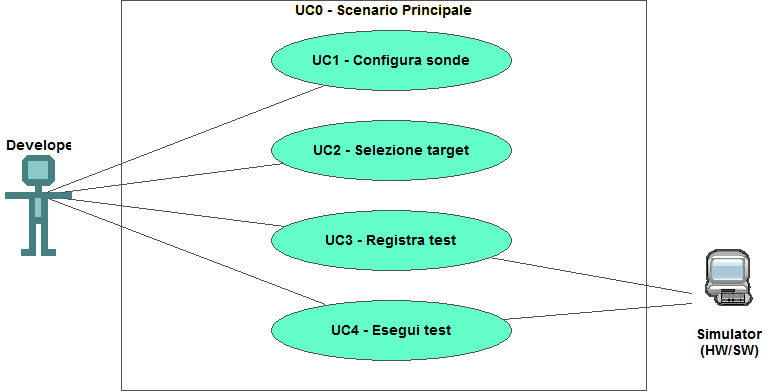
\includegraphics[width=0.9\columnwidth]{usecase/scenario-principale} 
    \caption{Use Case - UC0: Scenario principale}
\end{figure}

\begin{usecase}{0}{Scenario principale}
\usecaseactors{Sviluppatore applicativi}
\usecasepre{Lo sviluppatore è entrato nel plug-in di simulazione all'interno dell'IDE}
\usecasedesc{La finestra di simulazione mette a disposizione i comandi per configurare, registrare o eseguire un test}
\usecasepost{Il sistema è pronto per permettere una nuova interazione}
\label{uc:scenario-principale}
\end{usecase}

\section{Tracciamento dei requisiti}

Da un'attenta analisi dei requisiti e degli use case effettuata sul progetto è stata stilata la tabella che traccia i requisiti in rapporto agli use case.\\
Sono stati individuati diversi tipi di requisiti e si è quindi fatto utilizzo di un codice identificativo per distinguerli.\\
Il codice dei requisiti è così strutturato R(F/Q/V)(N/D/O) dove:
\begin{enumerate}
	\item[R =] requisito
    \item[F =] funzionale
    \item[Q =] qualitativo
    \item[V =] di vincolo
    \item[N =] obbligatorio (necessario)
    \item[D =] desiderabile
    \item[Z =] opzionale
\end{enumerate}
Nelle tabelle \ref{tab:requisiti-funzionali}, \ref{tab:requisiti-qualitativi} e \ref{tab:requisiti-vincolo} sono riassunti i requisiti e il loro tracciamento con gli use case delineati in fase di analisi.

\newpage

\begin{table}%
\caption{Tabella del tracciamento dei requisti funzionali}
\label{tab:requisiti-funzionali}
\begin{tabularx}{\textwidth}{lXl}
\hline\hline
\textbf{Requisito} & \textbf{Descrizione} & \textbf{Use Case}\\
\hline
RFN-1     & L'interfaccia permette di configurare il tipo di sonde del test & UC1 \\
\hline
\end{tabularx}
\end{table}%

\begin{table}%
\caption{Tabella del tracciamento dei requisiti qualitativi}
\label{tab:requisiti-qualitativi}
\begin{tabularx}{\textwidth}{lXl}
\hline\hline
\textbf{Requisito} & \textbf{Descrizione} & \textbf{Use Case}\\
\hline
RQD-1    & Le prestazioni del simulatore hardware deve garantire la giusta esecuzione dei test e non la generazione di falsi negativi & - \\
\hline
\end{tabularx}
\end{table}%

\begin{table}%
\caption{Tabella del tracciamento dei requisiti di vincolo}
\label{tab:requisiti-vincolo}
\begin{tabularx}{\textwidth}{lXl}
\hline\hline
\textbf{Requisito} & \textbf{Descrizione} & \textbf{Use Case}\\
\hline
RVO-1    & La libreria per l'esecuzione dei test automatici deve essere riutilizzabile & - \\
\hline
\end{tabularx}
\end{table}%             % Concept Preview
% !TEX encoding = UTF-8
% !TEX TS-program = pdflatex
% !TEX root = ../tesi.tex

%**************************************************************
\chapter{Progettazione e codifica}
\label{cap:progettazione-codifica}
%**************************************************************

\intro{Breve introduzione al capitolo}\\

%**************************************************************
\section{Tecnologie e strumenti}
\label{sec:tecnologie-strumenti}

Di seguito viene data una panoramica delle tecnologie e strumenti utilizzati.

\subsection*{Tecnologia 1}
Descrizione Tecnologia 1.

\subsection*{Tecnologia 2}
Descrizione Tecnologia 2

%**************************************************************
\section{Ciclo di vita del software}
\label{sec:ciclo-vita-software}

%**************************************************************
\section{Progettazione}
\label{sec:progettazione}

\subsubsection{Namespace 1} %**************************
Descrizione namespace 1.

\begin{namespacedesc}
    \classdesc{Classe 1}{Descrizione classe 1}
    \classdesc{Classe 2}{Descrizione classe 2}
\end{namespacedesc}


%**************************************************************
\section{Design Pattern utilizzati}

%**************************************************************
\section{Codifica}
             % Product Prototype
% !TEX encoding = UTF-8
% !TEX TS-program = pdflatex
% !TEX root = ../tesi.tex

%**************************************************************
\chapter{Verifica e validazione}
\label{cap:verifica-validazione}
%**************************************************************             % Product Design Freeze e SOP
% !TEX encoding = UTF-8
% !TEX TS-program = pdflatex
% !TEX root = ../tesi.tex

%**************************************************************
\chapter{Conclusioni}
\label{cap:conclusioni}
%**************************************************************

\section{Risultato ottenuto}
\begin{longtable}{lp{.48\textwidth}p{.15\textwidth}}
    \toprule
        \thcell{Id Requisito} & \thcell{Descrizione} & \thcell{Raggiunto}\\
        \midrule
        \endfirsthead
        % intestazione normale
        \multicolumn{3}{l}{\footnotesize\itshape
        Continua dalla pagina precedente} \\
        \toprule
        \thcell{Id Requisito} & \thcell{Descrizione} & \thcell{Raggiunto}\\
        %\midrule
        \endhead
        % piede normale
        %\midrule
        \multicolumn{3}{r}{\footnotesize\itshape
        Continua nella prossima pagina} \\
        \endfoot
        % piede finale
    \bottomrule
    \caption[Requisiti raggiunti]{Requisiti raggiunti}
    %\multicolumn{3}{r}{\footnotesize\itshape Si conclude dalla pagina precedente} 
    \\
    \endlastfoot
        RF1 & L'utente deve poter effettuare una ricerca all'interno del \gls{corpus} & Sì \\ \addlinespace
        RF2 & Implementazione di una collezione di test per valutare il sistema di ricerca mediante calcolo della precision, recall e f-measure& Sì \\ \addlinespace
        RF3 & Implementazione di una pagina di ricerca dei documenti all'interno del \gls{corpus} che utilizzi un tesauro generato manualmente & Sì\\ \addlinespace
        RF4 & Implementazione di una pagina di ricerca dei documenti all'interno del \gls{corpus} che utilizzi un \gls{autoencoder} & Sì\\ \addlinespace
        RF5 & Implementazione di una pagina di ricerca dei documenti all'interno del \gls{corpus} che utilizzi l'analisi della semantica latente & Sì\\ \addlinespace
        RF6 & Implementazione di una pagina di ricerca dei documenti all'interno del \gls{corpus} che utilizzi un \gls{autoencoder} & No\\ \addlinespace
        RF7 & Implementazione di una pagina di ricerca dei documenti all'interno del \gls{corpus} che utilizzi di un \gls{ensemble} dei metodi (tesauro manuale, tesauro automatico, analisi della semantica latente e \gls{autoencoder}) & No\\ \addlinespace
        RF8 & Implementazione di una pagina di ricerca dei documenti all'interno del \gls{corpus} che utilizzi un tesauro generico (di LibreOffice) & Sì\\ \addlinespace
        RF9 & I risultati delle ricerche devono essere aggregati per ID continui, quindi ordinati in base allo score & Sì \\ \addlinespace
        RF10 & Configurazione dello stemmer italiano & Sì \\ \addlinespace
        RV11 & Il prodotto deve essere eseguibile da browser (su Windows 10, browser Chrome $\geq$ 77.0.3865) & Sì \\ \addlinespace
        RQ12 & Deve essere fornita documentazione in inglese del codice in formato \gls{jsdoc} & Sì \\ \addlinespace
%%%%%% end data
\label{tabella:requisitiCompletati}
\end{longtable}
Non sono riuscito a completare tutti gli obiettivi prefissati all'inizio dello stage,
per le difficoltà emerse e già analizzate in §\ref{sec:problematiche}.
Anche se fossi riuscito ad implementare anche i restanti obiettivi, questo probabilmente
non avrebbe avuto un impatto nel miglioramento del recupero dell'informazione:
come evidenziato anche dal mio tutor aziendale, il \gls{corpus} era insufficiente
per riuscire ad estrarre efficacemente delle informazioni che potessero essere utili 
al fine del reperimento.

Si sarebbe potuto ottenere di più per esempio cercando di espandere il contesto
invece che di estrarre l'informazione dal \gls{corpus}: guardando in letteratura,
infatti, si possono trovare esempi (anche se pochi) che utilizzano le reti di Markov
e un contesto più ampio (Wikipedia in primis come fonte) su \gls{corpus} piccoli. 
Tale approccio però avrebbe richiesto uno sforzo sia dal punto di vista tecnologico (capire
come riadattare la libreria usata per il recupero dell'informazione o cercarne 
un'altra) che dal punto di vista di conoscenze mie (reti di Markov, in particolare),
non compatibile con i tempi dello stage. 

Ritengo sia più quello sono riuscito a ricevere dallo stage che quello che sono riuscito a dare a dare all'azienda: posso dire di portarmi a casa conoscenze in più, mentre l'azienda se non altro ha avuto la conferma che l'approccio naive è quello che ripaga di più (ed eventualmente di indagare verso un approccio probabilistico e non algebrico).

%*************************************************************
\section{Analisi critica del prodotto e del lavoro di stage}
%*************************************************************
\subsection{Conoscenze possedute e acquisite}
All'inizio dello stage, non avevo praticamente mai utilizzato Javascript (purtroppo appena accennato nel corso di tecnologie web e un aspetto secondario nel progetto). Avevo comunque una conoscenza di base di Python per implementare qualche esercizio di competitive programming e del corso di algoritmi e strutture dati e mi ha comunque permesso di provare ad applicare i primi concetti di recupero dell'informazione (p.es. calcolo di tf-idf) e confrontare le prestazioni della soluzione in Javascript con quella in Python.

Da questa esperienza ho imparato
\begin{itemize}
    \item il linguaggio di programmazione Javascript;
    \item delle basi di Node.js;
    \item i fondamenti del recupero dell'informazione;
    \item a utilizzare una libreria di calcolo scientifico in Javascript (LALOLib).
\end{itemize}

Se sono riuscito a reperire in autonomia il materiale necessario (cercando sia tra libri che paper) è anche per l'esperienza fatta durante il corso di studi.


%*************************************************************
\subsection{Utilizzazione del prodotto}
Il prodotto non era pensato per essere immediatamente utilizzabile, non interfacciandosi con quanto di esistente.
Per quanto riguarda la ricerca che fa uso dell'analisi della semantica latente, non è immediatamente utilizzabile in quanto le prestazioni della libreria in Javascript erano insufficienti anche per un \gls{corpus} di piccole dimensioni (circa 75 secondi per decomporre la matrice contro il mezzo secondo scarso di NumPy e i qualche manciata di centesimi di secondo con SciPy): purtroppo non ci sono alternative migliori in Javascript attualmente disponibili. 
Questi calcoli potrebbero essere effettuati lato server, ma comunque rimane una soluzione troppo inefficiente: specialmente se consideriamo che la quantità di testo trascritto è comunque relativamente piccola e corrisponde a circa 4 ore di filmato.

%*************************************************************
\subsection{Valutazione degli strumenti principalmente utilizzati}
\subsubsection{Javascript}
Meno banale di quello che potrebbe sembrare all'inizio: giusto per citare due particolarità, l'ereditarietà prototipale e le immediately invoked function expression. A volte lascia un po' troppe libertà. Mi ha sorpreso non trovare, tra le funzionalità "già incluse" (ovvero senza usare librerie esterne), una coda di priorità.

\subsubsection{lunr.js}
Semplice da usare se si conosce Javascript, ben documentato e lo sviluppo è attivo. Mi ha sorpreso positivamente e di poterlo riutilizzare in futuro. Di negativo c'è che non è ancora compatibile con i moduli di ES6\footnote{\url{https://github.com/olivernn/lunr.js/issues/401}}. 

\subsubsection{LALOLib}
Facile da utilizzare, discreta la documentazione e molto buono il supporto: anche se non troppo efficiente, le alternative non abbondano (se si deve utilizzare Javascript).     
%*************************************************************
\subsection{Possibili estensioni del prodotto}
Le estensioni possibili, più che nelle funzionalità, nell'approccio:
\begin{itemize}
    \item considerare come documenti non i singoli frammenti ma gruppi un po' più grandi di frammenti (bisogna però trovare il trade-off giusto tra numero di documenti e numero dimensione dei documenti singoli);
    \item provare a migliorare espandendo il contesto(p.es. con Wikipedia, come già accennato all'inizio del capitolo).
\end{itemize} 
             % Conclusioni
\appendix                               
% !TEX encoding = UTF-8
% !TEX TS-program = pdflatex
% !TEX root = ../tesi.tex

%**************************************************************
\chapter{Appendice A}
%**************************************************************

\epigraph{Citazione}{Autore della citazione}



             % Appendice A

%**************************************************************
% Materiale finale
%**************************************************************
\backmatter
\printglossaries
% !TEX encoding = UTF-8
% !TEX TS-program = pdflatex
% !TEX root = ../tesi.tex

%**************************************************************
% Bibliografia
%**************************************************************

\cleardoublepage
\chapter{Bibliografia}

\nocite{*}
% Stampa i riferimenti bibliografici
\printbibliography[heading=subbibliography,title={Riferimenti bibliografici},type=book]

% Stampa i siti web consultati
\printbibliography[heading=subbibliography,title={Siti web consultati},type=online]


\end{document}
